%%%%%%%%%%%%%%%%%%%%%%% file template.tex %%%%%%%%%%%%%%%%%%%%%%%%%
%
% This is a general template file for the LaTeX package SVJour3
% for Springer journals.          Springer Heidelberg 2010/09/16
%
% Copy it to a new file with a new name and use it as the basis
% for your article. Delete % signs as needed.
%
% This template includes a few options for different layouts and
% content for various journals. Please consult a previous issue of
% your journal as needed.
%
%%%%%%%%%%%%%%%%%%%%%%%%%%%%%%%%%%%%%%%%%%%%%%%%%%%%%%%%%%%%%%%%%%%
%
% First comes an example EPS file -- just ignore it and
% proceed on the \documentclass line
% your LaTeX will extract the file if required
\begin{filecontents*}{example.eps}
%!PS-Adobe-3.0 EPSF-3.0
%%BoundingBox: 19 19 221 221
%%CreationDate: Mon Sep 29 1997
%%Creator: programmed by hand (JK)
%%EndComments
gsave
newpath
  20 20 moveto
  20 220 lineto
  220 220 lineto
  220 20 lineto
closepath
2 setlinewidth
gsave
  .4 setgray fill
grestore
stroke
grestore
\end{filecontents*}
%
\RequirePackage{fix-cm}
%
%\documentclass{svjour3}                     % onecolumn (standard format)
%\documentclass[smallcondensed]{svjour3}     % onecolumn (ditto)
\documentclass[smallextended]{svjour3}       % onecolumn (second format)
%\documentclass[twocolumn]{svjour3}          % twocolumn
%
\smartqed  % flush right qed marks, e.g. at end of proof
%
\usepackage{graphicx}
\usepackage{todonotes}
%
% \usepackage{mathptmx}      % use Times fonts if available on your TeX system
%
% insert here the call for the packages your document requires
%\usepackage{latexsym}
% etc.
%
% please place your own definitions here and don't use \def but
% \newcommand{}{}
%
% Insert the name of "your journal" with
% \journalname{myjournal}
%
\begin{document}

\title{Silico-Paleontogy%\thanks{Grants or other notes
%about the article that should go on the front page should be
%placed here. General acknowledgments should be placed at the end of the article.}
}
\subtitle{Visualizing genetic programming ancestries with graph databases}
% \subtitle{Digging through the relics of artificial evolution}

%\titlerunning{Short form of title}        % if too long for running head

\author{Nicholas Freitag McPhee         \and
        Thomas Helmuth \and
        Lee Spector \and
        Maggie Casale \and
        Mitch Finzel \and
        Any Others? %etc.
}

%\authorrunning{Short form of author list} % if too long for running head

\institute{N. McPhee \at
              Division of Science and Mathematics \\
              University of Minnesota, Morris \\
              Morris, MN USA \\
              Tel.: +320-589-6320\\
              \email{mcphee@moris.umn.edu}           %  \\
%             \emph{Present address:} of F. Author  %  if needed
           \and
           S. Author \at
              second address
}

\date{Received: date / Accepted: date}
% The correct dates will be entered by the editor


\maketitle

\begin{abstract}
	Much evolutionary computation research collects and reports thin statistical
	summaries that fail to capture or convey the complex dynamics of our
	actual runs, and all their micro-level events. In principle, however, we control
	every moment in our evolutionary runs and could record all these events.
	This would, for example, allow us to build full ancestry trees, identifying and analyzing the key events that led to success in a run, or blocked it. Here we
	illustrate the use of graph databases to collect rich details from genetic programming runs, and then describe information rich visualizations designed to aid in the understanding of these large, complex data sets.
	These visualizations have been key in discovering surprising and significant
	events in our runs, leading to new understanding of the dynamics of our
	evolutionary systems.
\keywords{Genetic programming \and Visualization \and Ancestries \and Graph databases}
% \PACS{PACS code1 \and PACS code2 \and more}
% \subclass{MSC code1 \and MSC code2 \and more}
\end{abstract}

\section*{Outline}
\marginpar{Obviously this has to go away.}

My general idea for the outline:
\begin{enumerate}
	\item Introduction: Rant about throwing away all that data and talk about why that's a bummer. This will actually probably be pretty long, maybe long enough that it should be a separate section?
	\item Graph Databases: Describe the basic idea, and our particular (current) data schema (include the semantics).
	\item Visualizations: Describe different edges, boxes sizes and shapes, colors (even though they won't display here)
	\begin{enumerate}
		\item Full runs
		\item Just ancestors
		\item Filtered by genes
	\end{enumerate}
	\item What have we learned? Hyperselection. Semantics hyperselection. Use the end of the poster run to illustrate both of these features.
	\item Conclusions: Graph DBs make this work possible and more people should do it. Does suck up a lot of disk space and takes a while, though, so there's work to be done. Need to get better at automating processes and combining analysis across multiple runs.
\end{enumerate}

\section{Introduction}
\label{sec:intro}

\begin{quote}
	In order to discover the actual steps by which the male of any existing 
	bird has acquired his magnificent colours or other ornaments, we ought 
	to behold the long line of his extinct progenitors; \emph{but this is obviously impossible}.\footnote{Emphasis ours.} \\
	\\
	--- Charles Darwin, in reference to peacocks~\cite{Darwin} 
\end{quote}

After people began to realize that species were not fixed, and that the fossil 
record contained evidence of a long and complex natural history, it also
became clear that this record was terribly incomplete. In the quote above
Darwin clearly realized the potential value of a complete ancestral record in
understanding evolutionary processes, but he also took it as a given that
such a record was not to be had.

The incompleteness of historical record, both human and natural, continues
to challenge scholars in a host of fields. Paleontologists work with a 
profoundly
incomplete fossil record, often describing and classifying entire categories of
organisms based a few teeth. The human historical record is no more complete,
with numerous valuable resources lost to the ravages of time. Worse, these 
gaps are often neither random nor symmetric, substantially skewing our view 
of that history. Teeth, for example, are often all we have of ancient 
sharks and their kin because their skeletons are made of cartilage, which
typically doesn't fossilize.

While it was impossible for Darwin to ``behold the long line of \ldots 
[peacock] progenitors'', in evolutionary computation it is in principle possible
to save \emph{all} the data from a run, and indeed explore all the progenitors
of a successful individual. As described in Section~\ref{sec:EC_pattern},
however, we rarely collect and analyze this type of data, instead only sharing
thin statistically summaries, pale shadows of the extremely complex 
processes that stand behind our research. 
In this paper, however, we propose
saving far more data tha has been common in the field, recording all the ``little'' low-level events that ultimately drive whatever large-scale trends 
we observe in our runs.

This does, however, represent a substantial increase in the amount of data
collected, which means that we need tools and techniques to store, explore,
analyze, and share results from that data. In recent work~\cite{graph_db_work}
we have found graph databases (discussed in
Section~\ref{sec:graph_DBs}) to be an effective tool for managing the 
substantial collection of data generated during a run. 

Visualizations are central to the success
of our work with graph databases, and Section~\ref{sec:visualizations}
describes our design of data rich 
visualizations that allow us to effectively explore and share results such as
complex ancestry graphs. We will then share examples of things we've learned
from such ancestry graphs in Section~\ref{sec:learned}, and present conclusions
and ideas for future work in Section~\ref{sec:conclusions}.

\todo[inline]{I don't currently reference the Related Work section in the
roadmap, and I feel like I probably should. Not sure where/how, though.}

\section{Related work}
\label{sec:related}

We are not aware of any other work in evolutionary computation using graph
databases to store and analyze full ancestry trees in a systematic way. That
said, there is other work where ancestry information has been collected,
analyzed, and visualized.

\todo[inline]{Crib stuff from, e.g., the VizGEC paper in Denver.}

\section{A common pattern in EC research}
\label{sec:EC_pattern}

\section{Graph databases}
\label{sec:graph_DBs}

\section{Visualizations}
\label{sec:visualizations}

\section{What have we learned?}
\label{sec:learned}

\section{Conclusions}
\label{sec:conclusions}

\todo[inline]{We may want a separate future work section? Not sure.}

\section*{Random examples from Springer}

\todo[inline]{This is all stuff from Springer and needs to be removed.}

Text with citations \cite{RefB} and \cite{RefJ}.

\subsection{Subsection title}
\label{sec:2}
as required. Don't forget to give each section
and subsection a unique label (see Sect.~\ref{sec:1}).
\paragraph{Paragraph headings} Use paragraph headings as needed.
\begin{equation}
a^2+b^2=c^2
\end{equation}

% For one-column wide figures use
\begin{figure}
% Use the relevant command to insert your figure file.
% For example, with the graphicx package use
  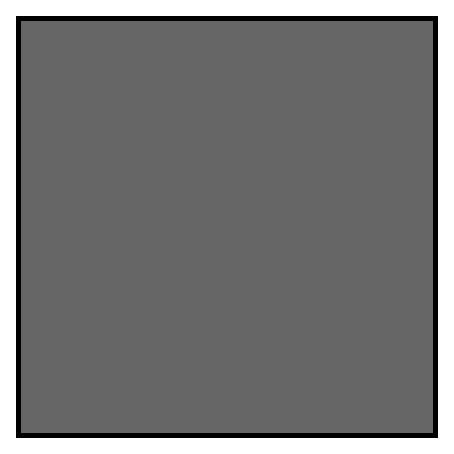
\includegraphics{example.eps}
% figure caption is below the figure
\caption{Please write your figure caption here}
\label{fig:1}       % Give a unique label
\end{figure}
%
% For two-column wide figures use
\begin{figure*}
% Use the relevant command to insert your figure file.
% For example, with the graphicx package use
  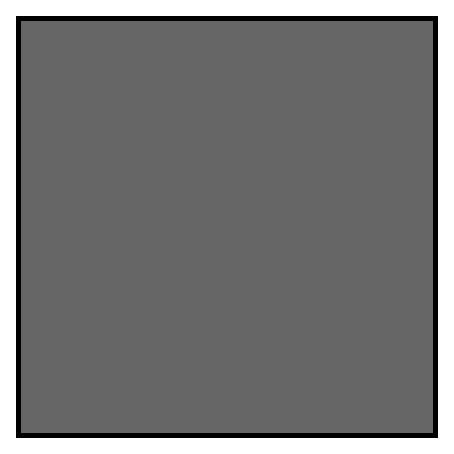
\includegraphics[width=0.75\textwidth]{example.eps}
% figure caption is below the figure
\caption{Please write your figure caption here}
\label{fig:2}       % Give a unique label
\end{figure*}
%
% For tables use
\begin{table}
% table caption is above the table
\caption{Please write your table caption here}
\label{tab:1}       % Give a unique label
% For LaTeX tables use
\begin{tabular}{lll}
\hline\noalign{\smallskip}
first & second & third  \\
\noalign{\smallskip}\hline\noalign{\smallskip}
number & number & number \\
number & number & number \\
\noalign{\smallskip}\hline
\end{tabular}
\end{table}


%\begin{acknowledgements}
%If you'd like to thank anyone, place your comments here
%and remove the percent signs.
%\end{acknowledgements}

% BibTeX users please use one of
\bibliographystyle{spbasic}      % basic style, author-year citations
%\bibliographystyle{spmpsci}      % mathematics and physical sciences
%\bibliographystyle{spphys}       % APS-like style for physics
\bibliography{GPEM_viz.bib}   % name your BibTeX data base

\end{document}
% end of file template.tex

